\documentclass[../../main.tex]{subfiles}


\begin{document}
\subsection*{(a)}
We can split the event log into two event logs using the plugin 'Filter Log on Event Attribute Values' with the following selections:\\
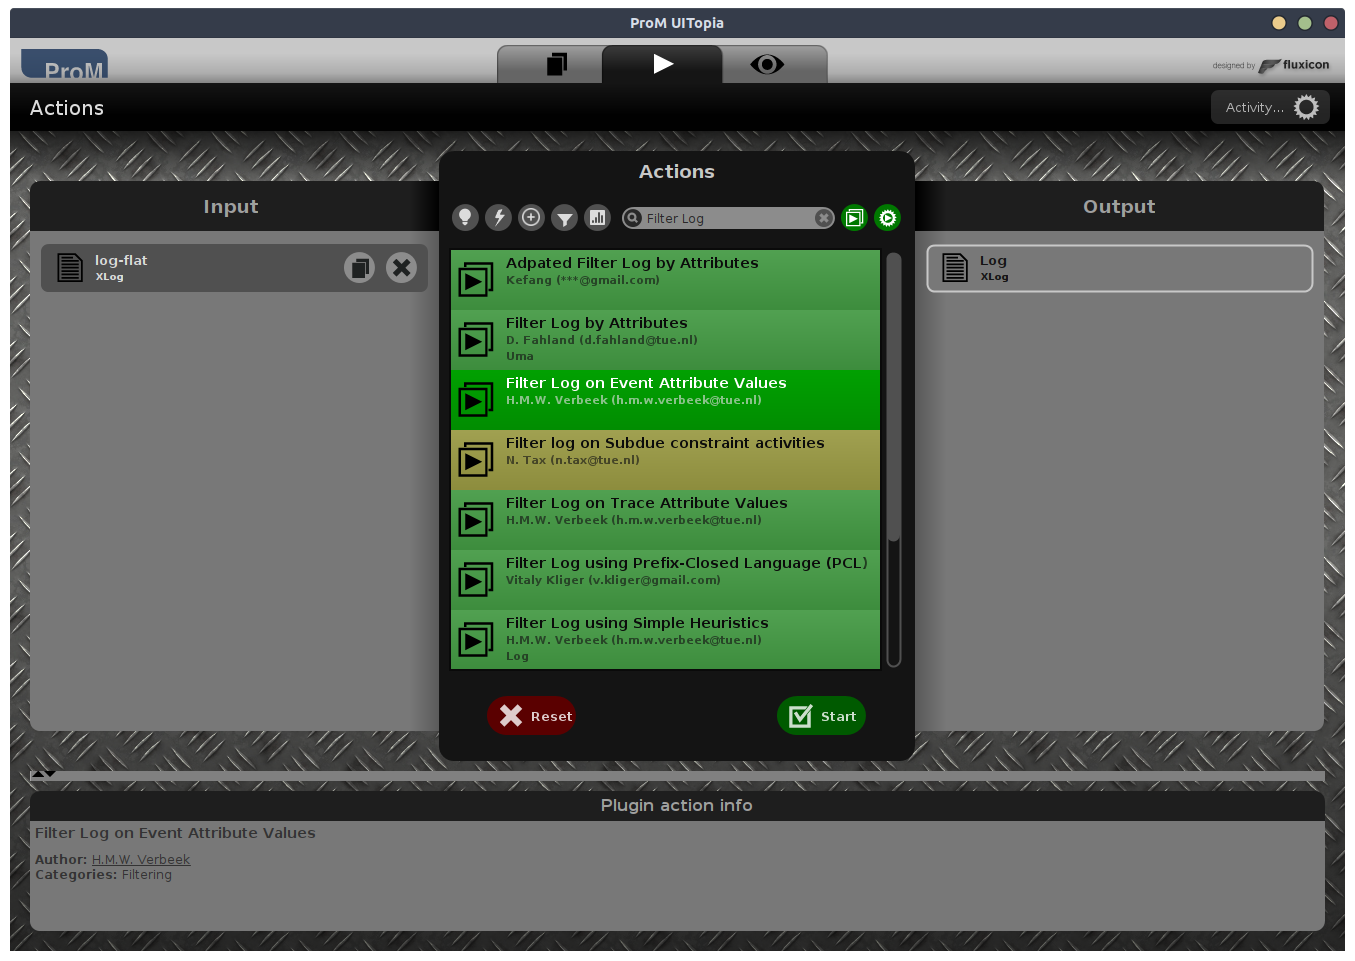
\includegraphics[width=0.33\columnwidth]{img/ProM_a_plugin.png}
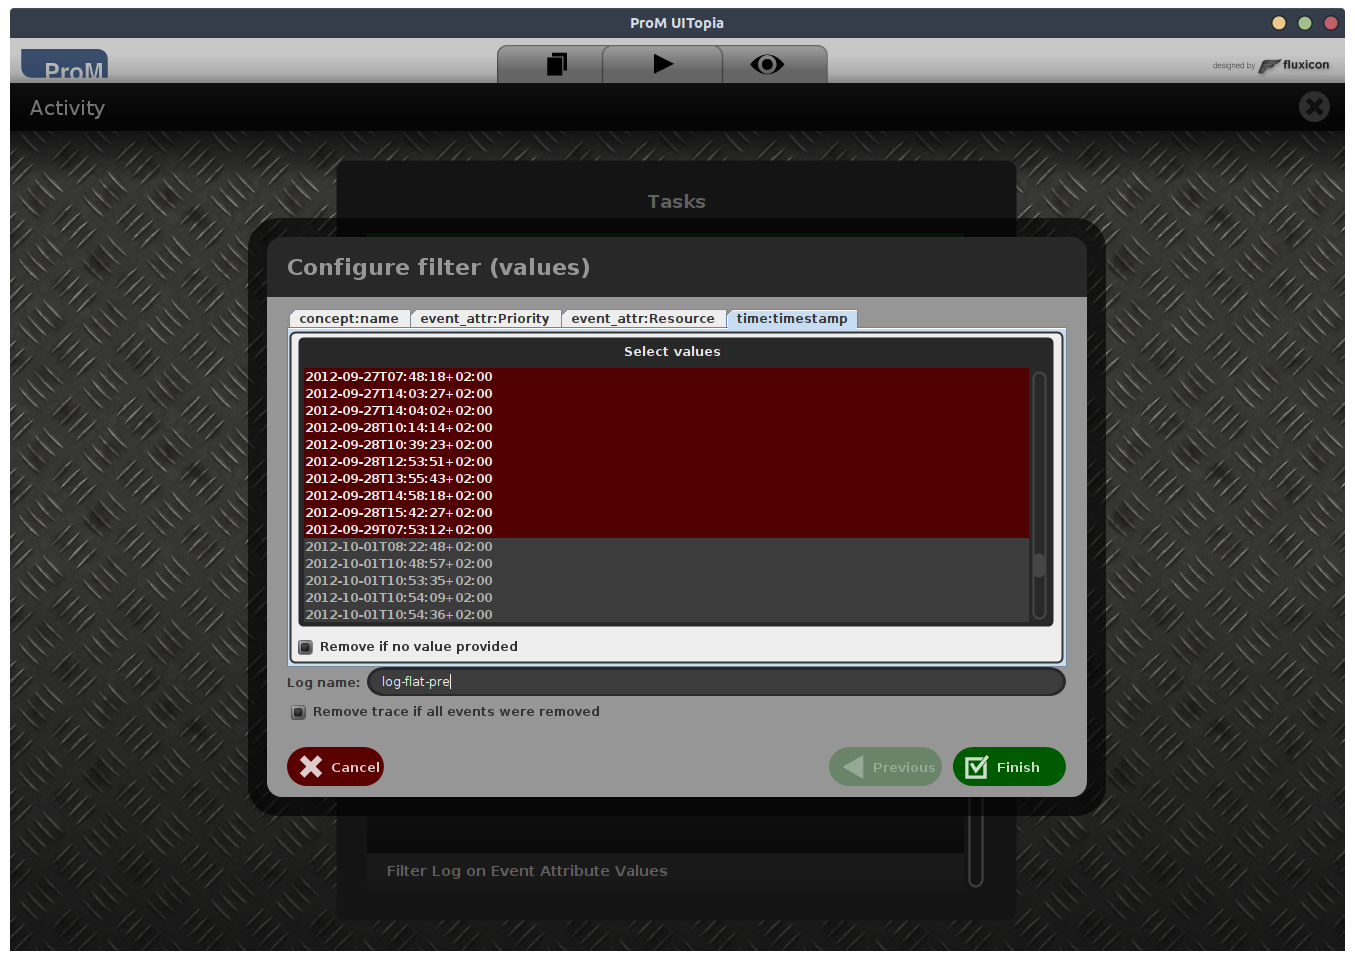
\includegraphics[width=0.33\columnwidth]{img/ProM_a_pre_method.png}
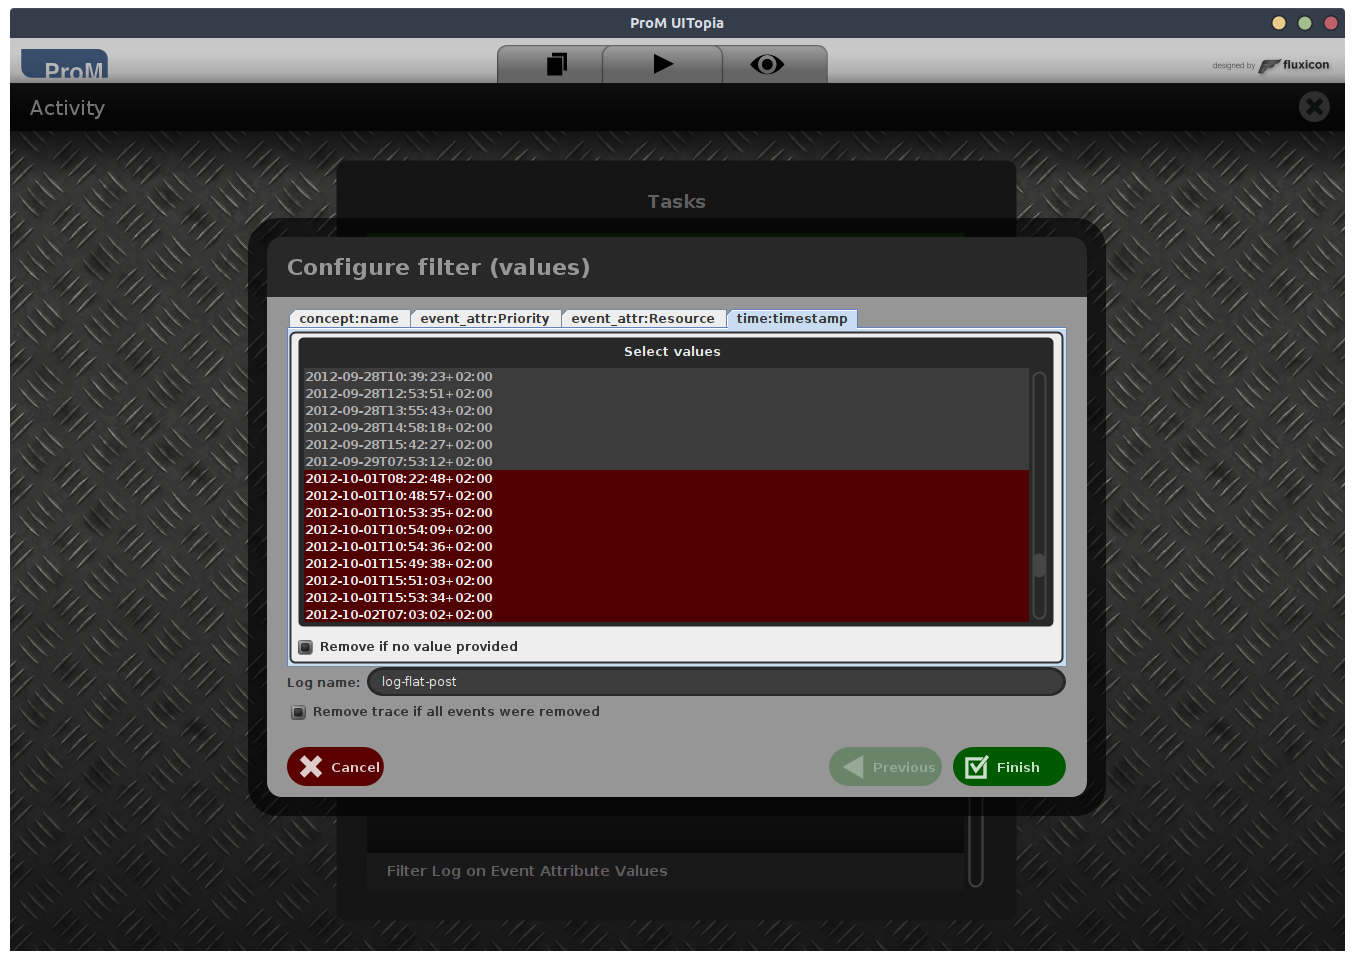
\includegraphics[width=0.33\columnwidth]{img/ProM_a_post_method.png}\\
Afterwards, we can apply our filtering to only allow valid traces, as seen before.\\

For the event log pre 01.10.2012 we get 13 unique activities across 3708 cases, as a whole consisting of 6 variants. \\
For the event log post (including) 01.10.2012 we get 12 unique activities across 730 cases, as a whole consisting of 6 variants. \\
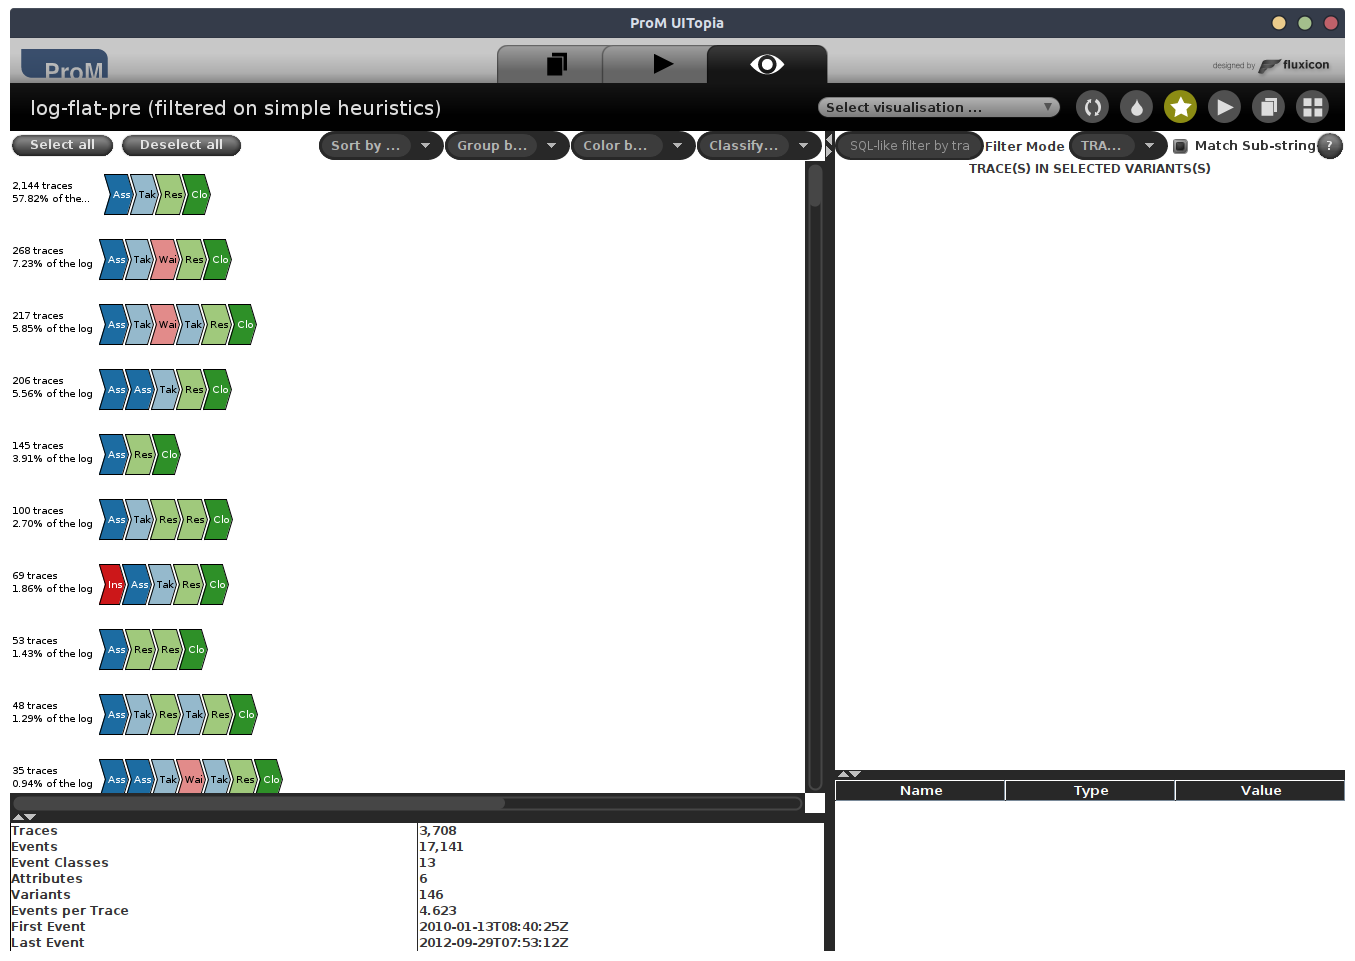
\includegraphics[width=0.5\columnwidth]{img/ProM_a_pre_traces.png}
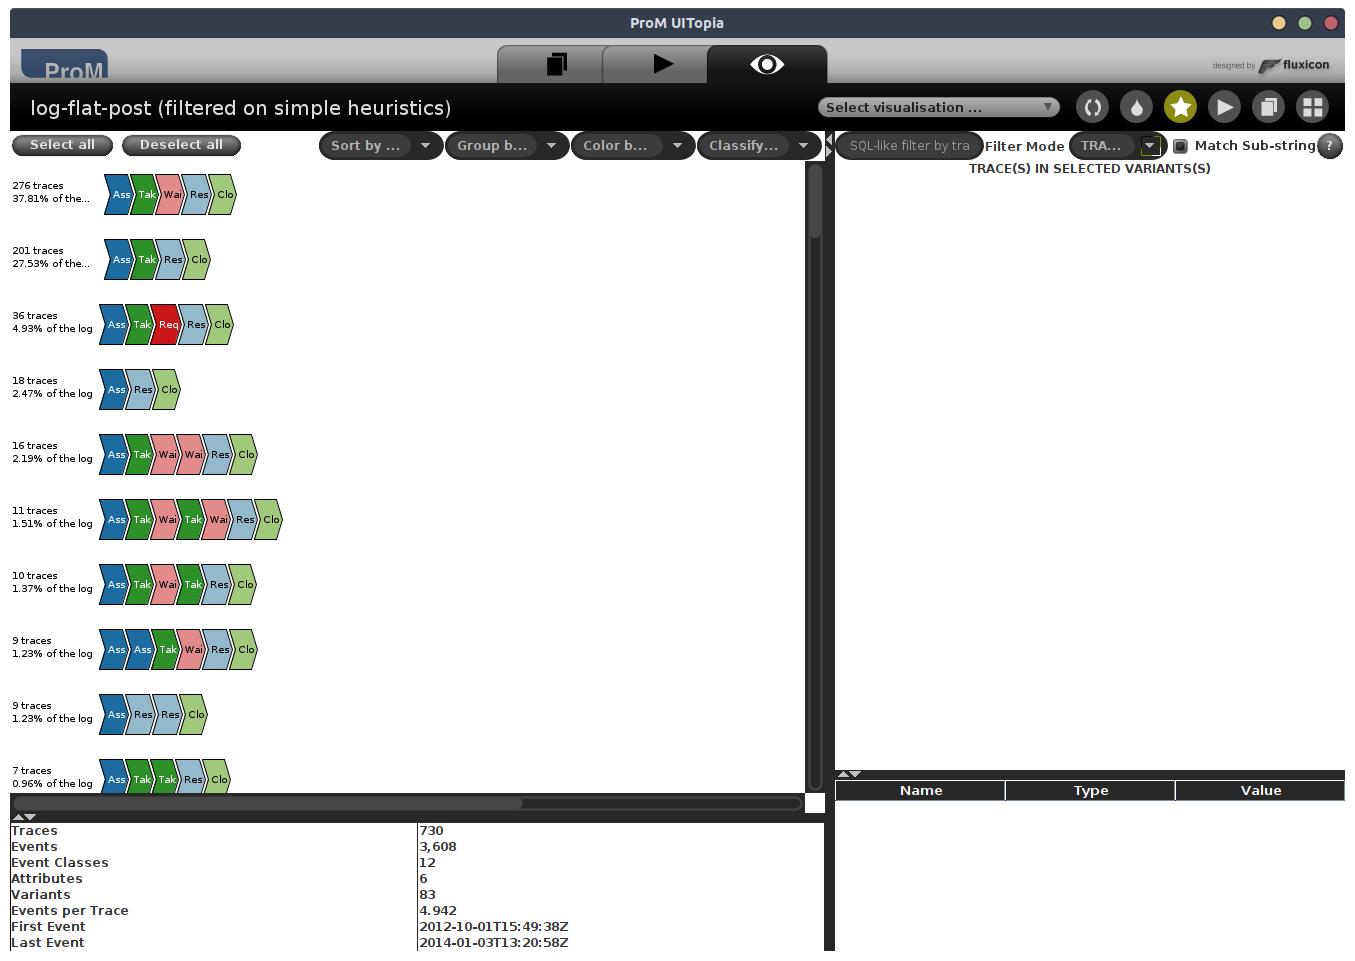
\includegraphics[width=0.5\columnwidth]{img/ProM_a_post_traces.png}\\

\subsection*{(b)}
1. We apply the following workflow both for \textit{log-pre-complete} and \textit{log-post-complete}:
\begin{enumerate}
\item Apply plugin 'Interactive Data-aware Heuristic Miner (iDHM)'
\item Set 'Options \& Thresholds' to\\
\begin{table}[h!]
\begin{tabular}{l|llll}
           & i) (\textit{log-pre-complete}) & ii) (\textit{log-pre-complete}) & iii) (\textit{log-post-complete}) & iv) (\textit{log-post-complete})\\
           \hline
Frequency  & 0.1 & 0   & 0.1  & 0   \\
Dependency & 0.9 & 0.9 & 0.9  & 0.9 \\
Bindings   & 0.1 & 0.1 & 0.1  & 0.1 \\
Conditions & 0.5 & 0.5 & 0.5  & 0.5
\end{tabular}
\end{table}
All tasks connected: True
\item Select 'Petri net' as 'Output: Process Model' and click 'Export model'
\item Use the log and the newly created Petri net as input for the 'Multi-perspective Process Miner' plugin
\end{enumerate}
This results in the following Models:\\
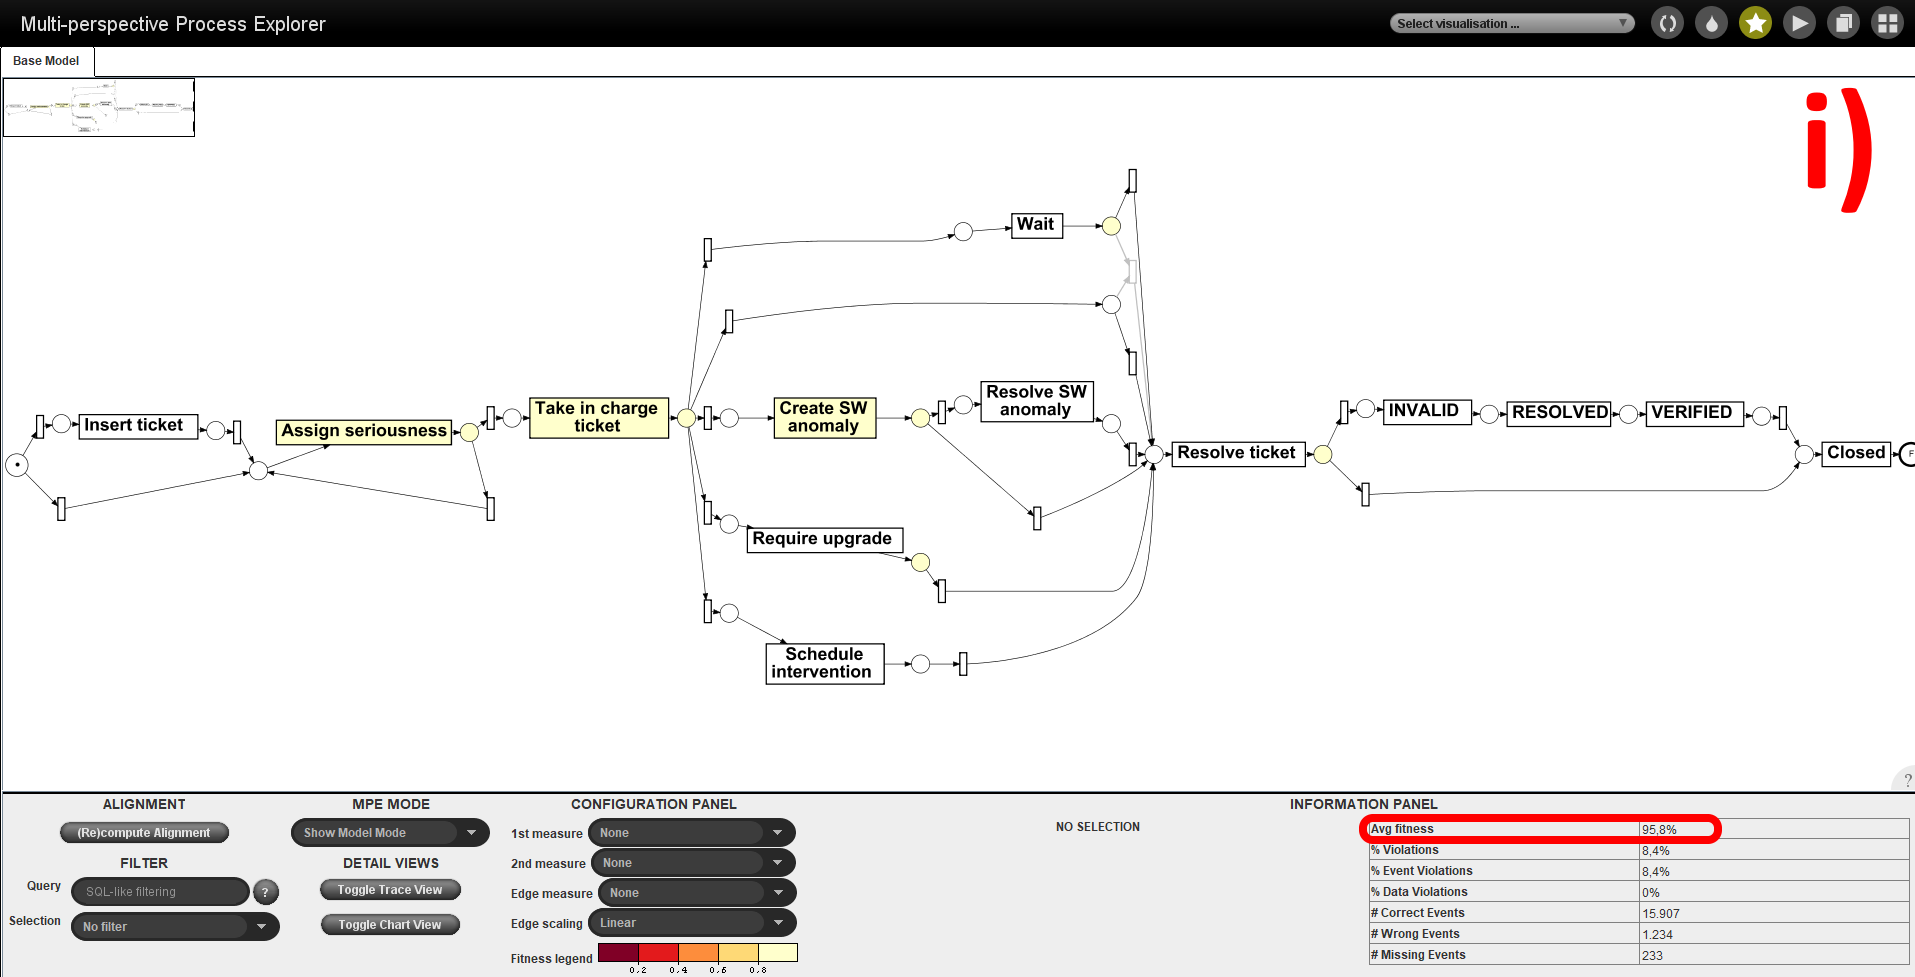
\includegraphics[width=0.5\columnwidth]{img/ProM_b_1i.png}
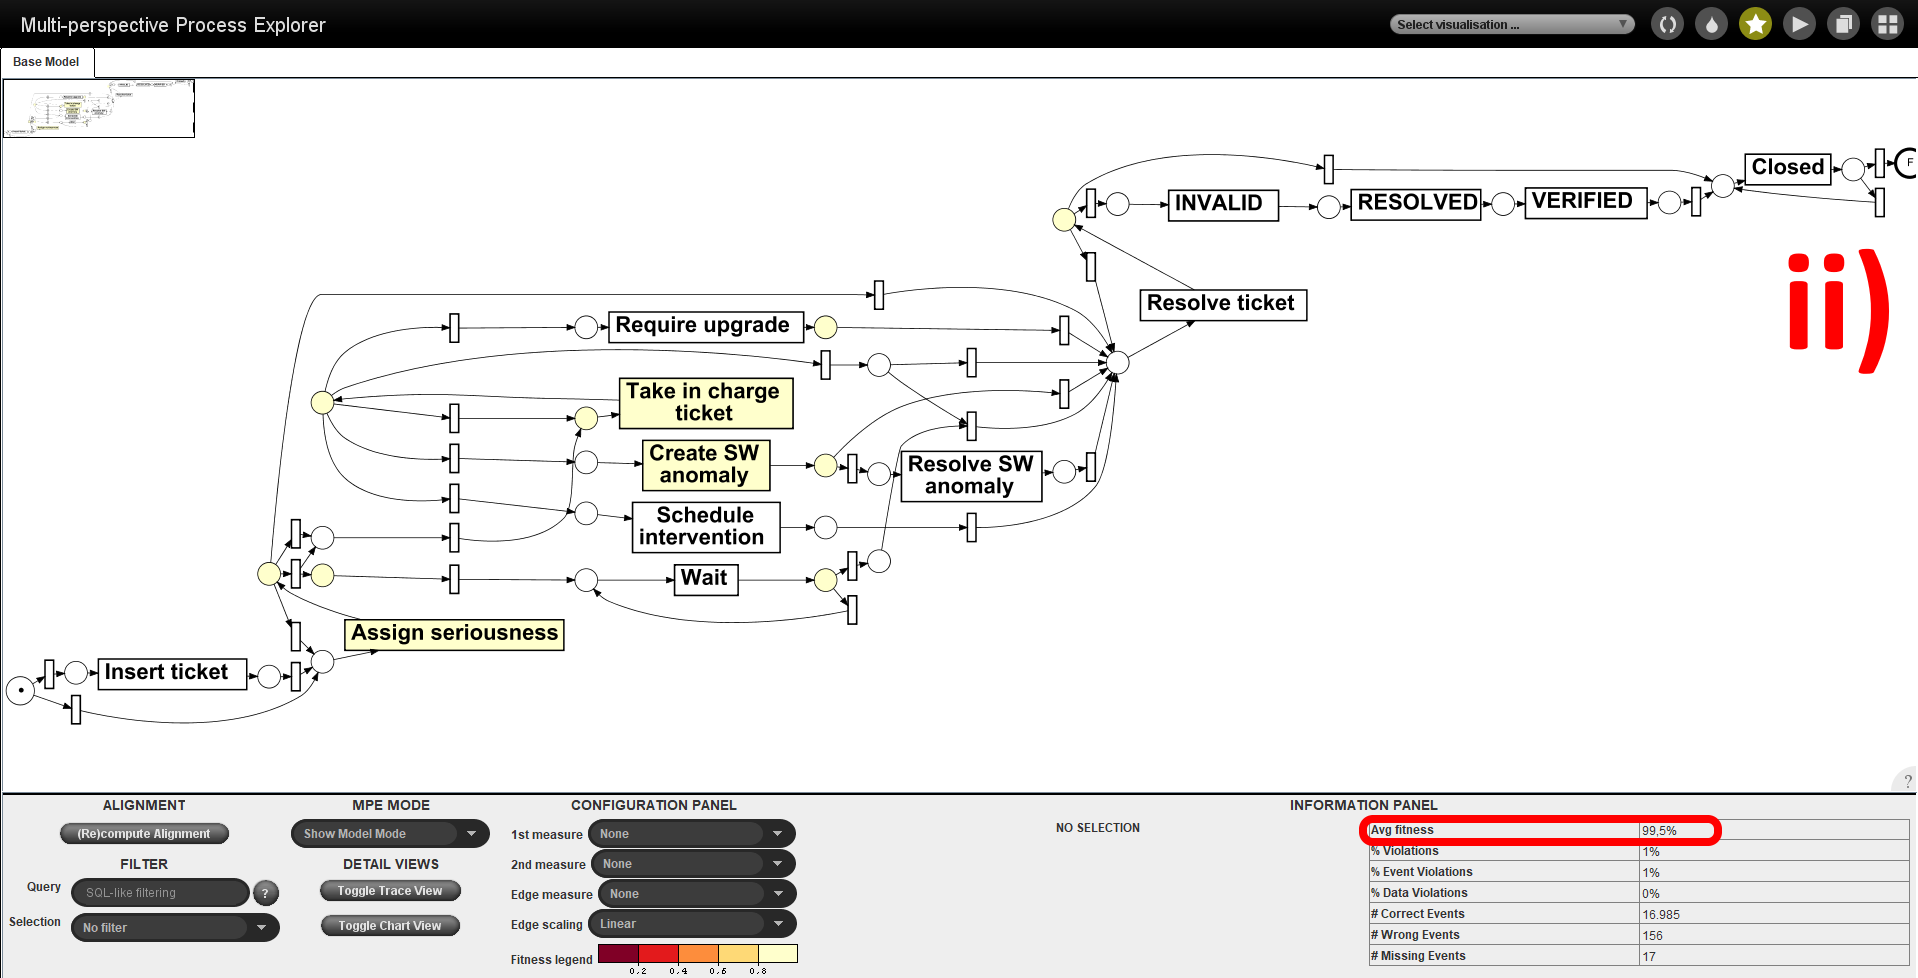
\includegraphics[width=0.5\columnwidth]{img/ProM_b_1ii.png}
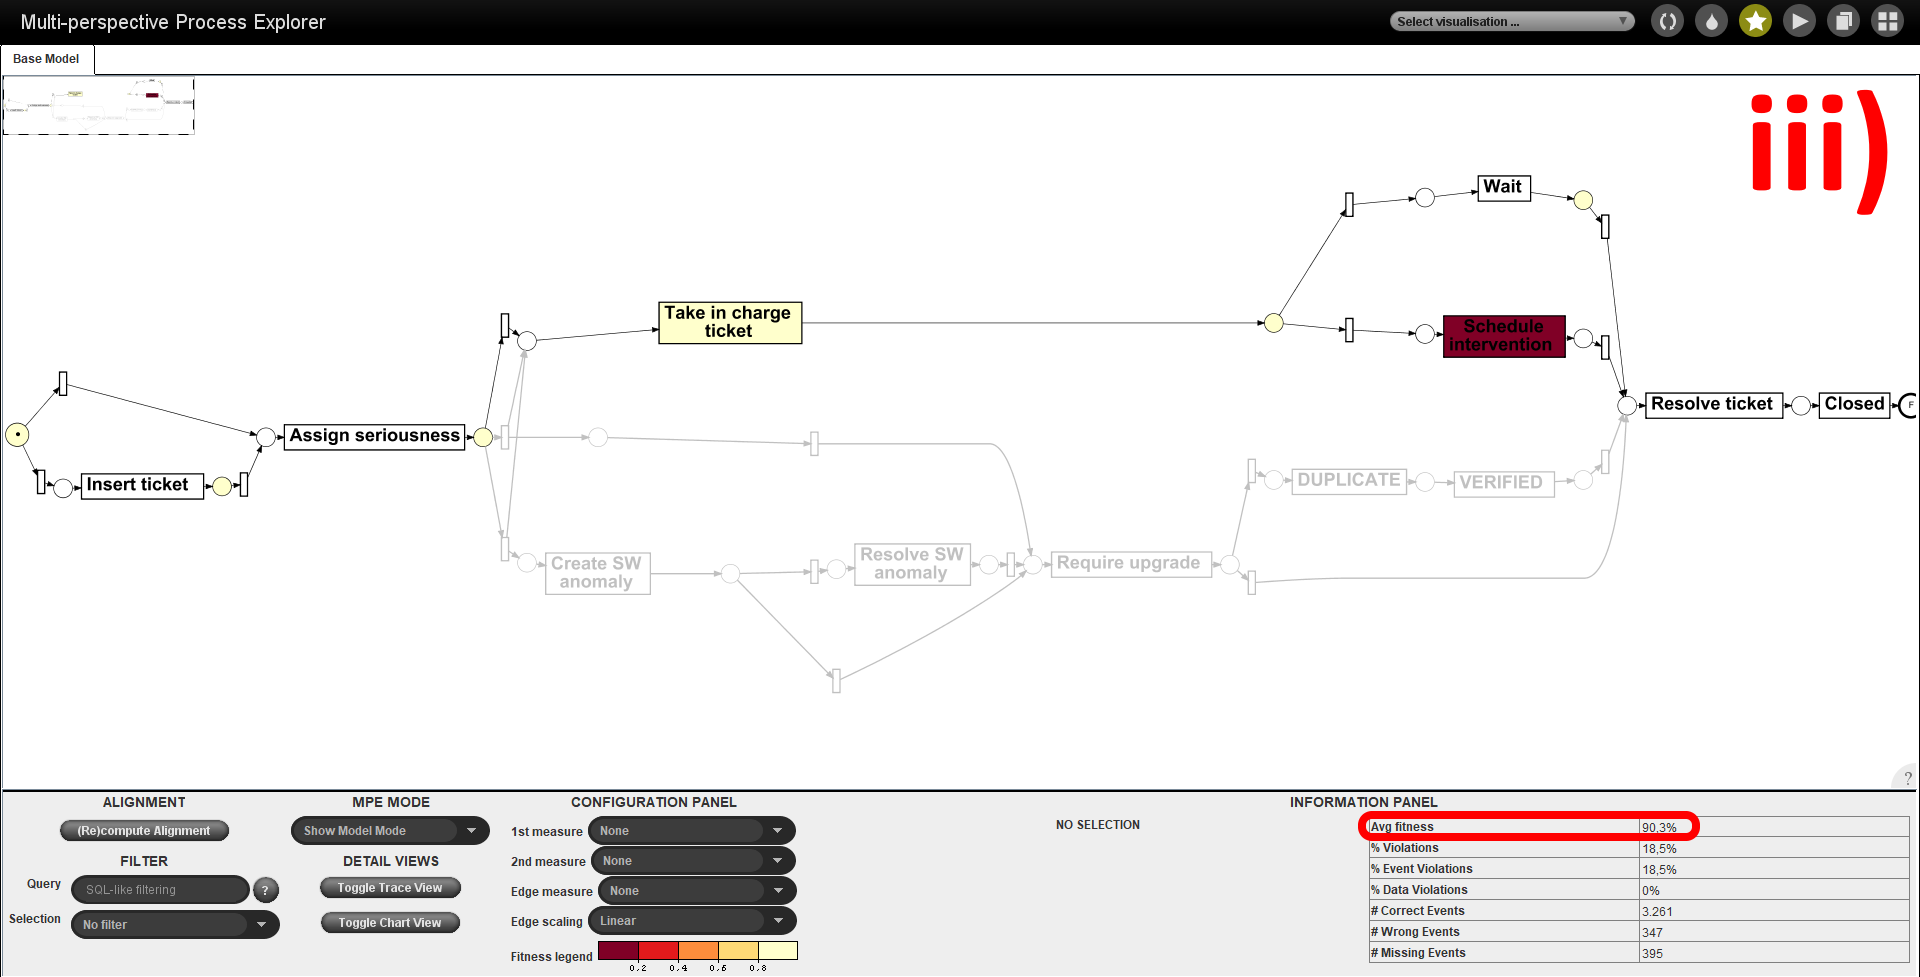
\includegraphics[width=0.5\columnwidth]{img/ProM_b_1iii.png}
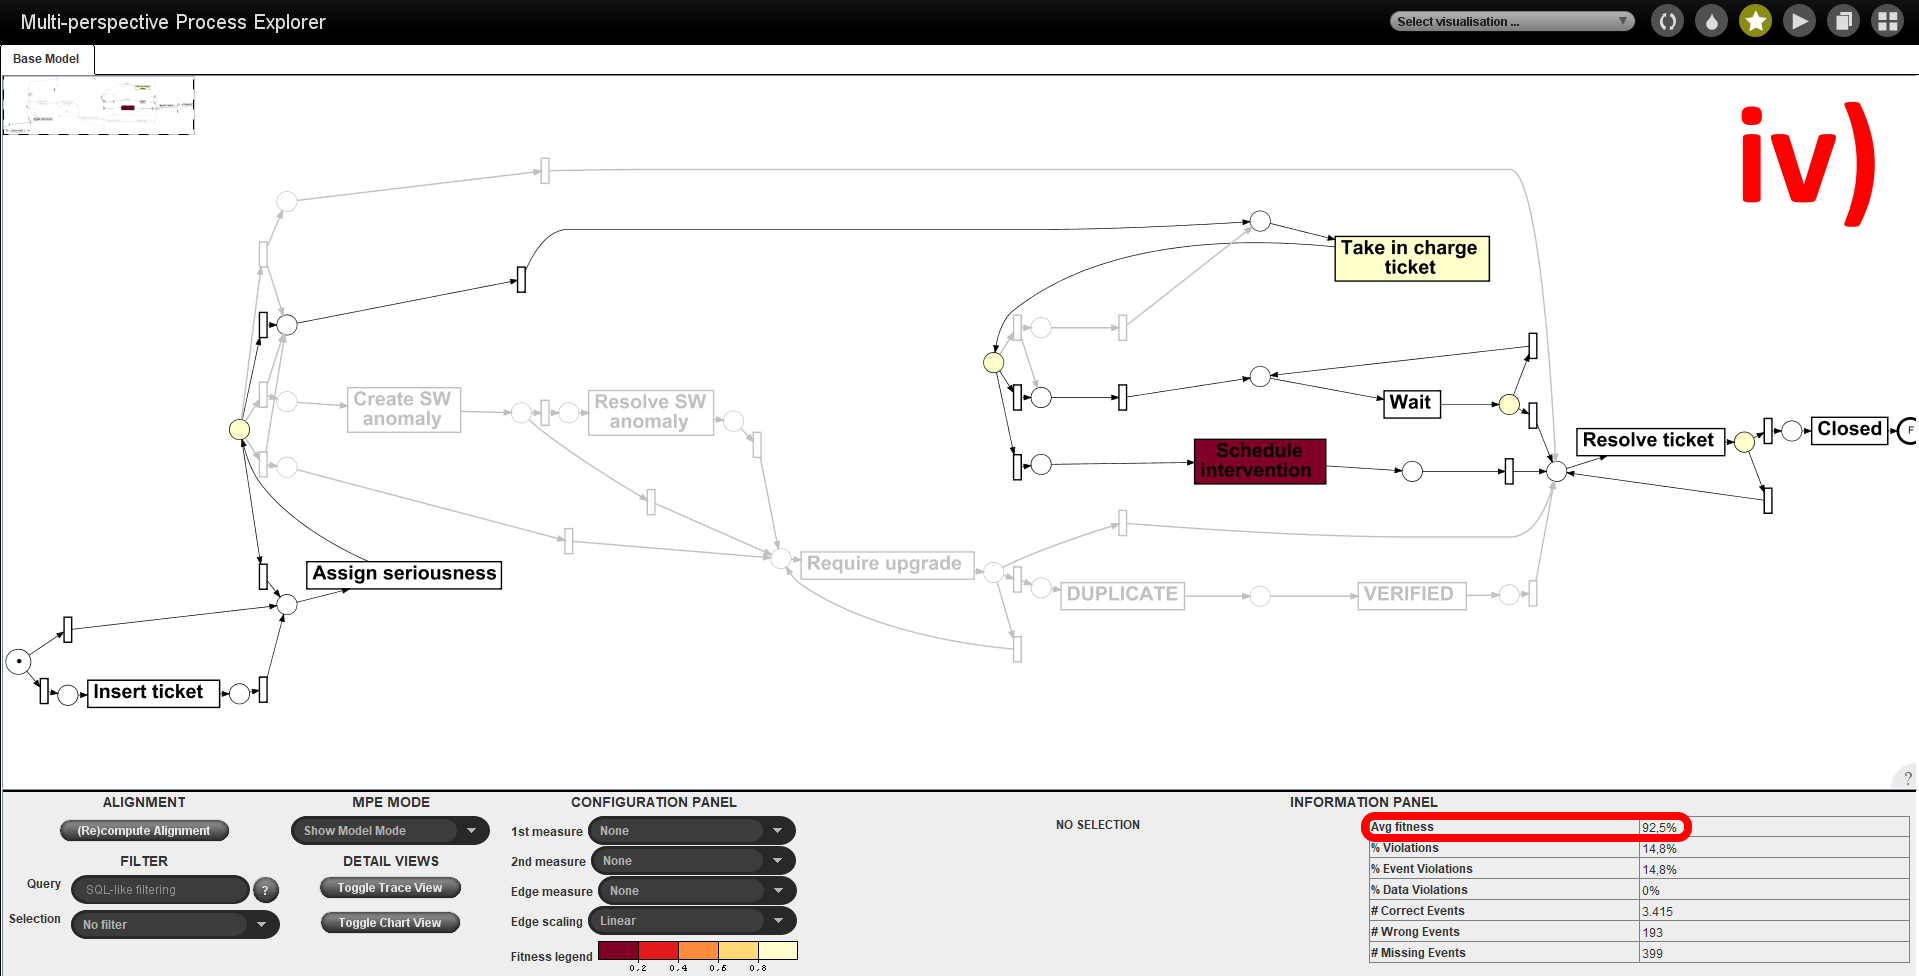
\includegraphics[width=0.5\columnwidth]{img/ProM_b_1iv.png}
As we can see all these models exceed our fitness threshold of 90\% and contain all activities occuring in their respective logs (\textit{log-pre-complete} doesn't contain the activity DUPLICATE and \textit{log-post.complete} doesn't contain the activities INVALID and RESOLVED).

\subsection*{(c)}
\begin{enumerate}
\item We visualized the three most frequent trace variant and their frequencies with the Explore Event Log utility of ProM. We got these three results:\\
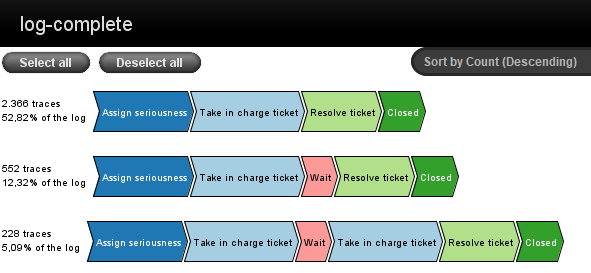
\includegraphics[width=0.5\columnwidth]{img/ProM_explore_log_complete.png}
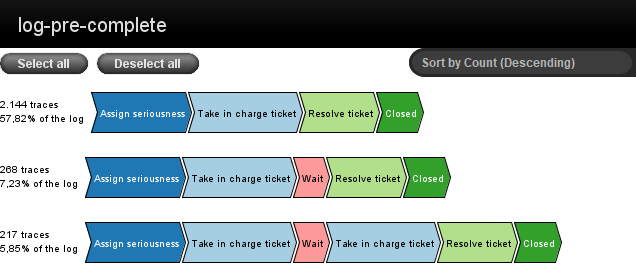
\includegraphics[width=0.5\columnwidth]{img/ProM_explore_log_pre.png}
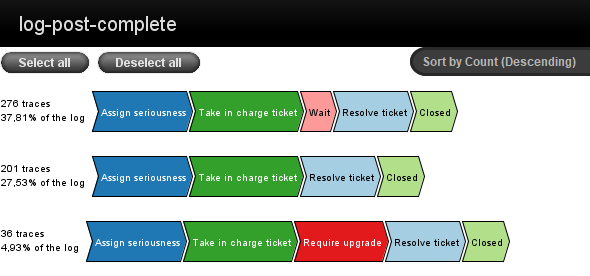
\includegraphics[width=0.5\columnwidth]{img/ProM_explore_log_post.png}\\
The first similarity observed between the three most frequent trace variants of all three event logs is, that they all start with the Assign seriousness and Take in charge ticket activities and finish with Resolve ticket and Closed. The second observation is the equality of the three most frequent trace variants of the \textit{log-complete} and \textit{log-pre-complete} event logs. This makes sense since most of the events of \textit{log-complete} are in \textit{log-pre-complete} and not in \textit{log-post-complete}. This also explains the difference in absolute frequency of the most common trace variant between \textit{log-complete} and \textit{log-pre-complete} and the most frequent one of \textit{log-post-complete} which differ by one order of magnitude. Another important difference is that in \textit{log-complete} and \textit{log-pre-complete} the most common trace variant has a relative frequency of over $50\%$ whilst in \textit{log-post-complete} the most common trace variants are more equally diveded between the two most frequent traces with $38\%$ and $28\%$. Finally the activity Require upgrade is only present in the three most common trace variants in the \textit{log-post-complete} event log.
\item All trace variants are replayable on both models:\\
\begin{tabular}{c | c c c}
    & $\sigma_{compl}$ & $\sigma_{pre}$ & $\sigma_{post}$ \\
    \hline
    $M_{pre}$ & $\langle$Assign seriousness, & $\langle$Assign seriousness, & $\langle$Assign seriousness, \\
    & Take in charge ticket, & Take in charge ticket, & Take in charge ticket, \\
    & Resolve ticket, & Resolve ticket, & Wait \\
    & Closed$\rangle$ & Closed$\rangle$ & Resolve ticket, \\
    & & & Closed$\rangle$ \\
    $M_{post}$ & $\langle$Assign seriousness, & $\langle$Assign seriousness, & $\langle$Assign seriousness, \\
    & Take in charge ticket, & Take in charge ticket, & Take in charge ticket, \\
    & Resolve ticket, & Resolve ticket, & Wait \\
    & Closed$\rangle$ & Closed$\rangle$ & Resolve ticket, \\
    & & & Closed$\rangle$ \\
\end{tabular}
\end{enumerate}


\subsection*{(d)}

\end{document}